\documentclass[../main.tex]{subfiles}

\begin{document}

\chapter{Introduction}\label{sec:introduction}
The increase of computation and dissemination of computing devices in recent years ($\sim$ 15 years) is undeniable.
Devices with same (or greater) computation power that took the man to the moon is today in a hand's reach and many are used to control machines everywhere.

With this increase on computation power, we can now solve some problems that were not solvable in a reasonable time in the past, thus the \emph{renaissance} of some optimization based methods, such as Neural networks and Artificial Intelligence.

For other more common methods such \mpc~\cite{GarciaEtAl1989}, this development meant solving more significant problems in less time, sometimes even in real-time~\cite{BesselmannEtAl2008}, and using small computation units smaller than coins~\cite{BanguraMahony2014}.

Consequently the list of possible applications of \mpc{}, increased, instead of using for single equipments in petrochemical plants with large time scales, to control system with scale of districts and cities such as \wdns~\cite{ZhangEtAl2021} and \dhns~\cite{TaylorEtAl2021}.
This presents a gradual insertion of \mpc{} into \cps{}, in which computers and physical machines are tightly coupled.

Nevertheless, for some large-scale systems, the calculation with multiple decision variables may still be expensive.
Needing some subterfuges, such as distributing it into different computation units and making them communicate.
As we will see, this strategy is called \dmpc and come in many flavors.

However, as we will see, not so many studies have been made on the security of the \dmpc{} strategies when units do not communicate honestly.
This work, however, studies what happens when computation units do not work cooperatively in a \dmpc{} framework.

To give a perspective to a general reader on how it can affect the daily life, we tell a simple qualitatively example in form of a story. The conclusion will serve as a main take-away of the possible effects of non-cooperative behaviors.
\newpage
\section{When greediness backfires}
6 o'clock on a Christmas morning.
You wake up.
Shivering.
The tips of your fingers are blue, and you ask yourself why you accepted to make part of this housing project.

The housing project was set in an undisclosed place to test a new sustainable \dhn{}.
Engineers from around the world were invited to take part in the project for one year to test drive the \dhn{} and file bugs.

Nourishment and all other amenities would be paid for.
So you willingly accepted.
What could go wrong?

It seemed okay-ish until $6$ weeks ago, when the days became shorter and shorter and the air colder and colder.

You climb out of bed and look at your house's central temperature control indicator. The outside temperature is $-5^{o}$C, and the mean temperature inside is $7^{o}$C.
The thermostat is still on, indicating that the comfortable $23^{o}$C you set yesterday was still saved. However, you see a flashing dim orange light in the corner of your eye. A small LED panel indicating:
\begin{quote}
ERR706
\end{quote}

Something is wrong.
This is the first time you have seen this message, and it is the last week of the project.
You look at your house, trying to find the manual given on your first day. Nada!

You take your coat, put on some gloves, and look outside your window.
You observe the centralized heat provider unit in the middle of the \emph{cul-de-sac} you live.
A similar orange light is flashing.
\begin{figure}[H]
  \centering
  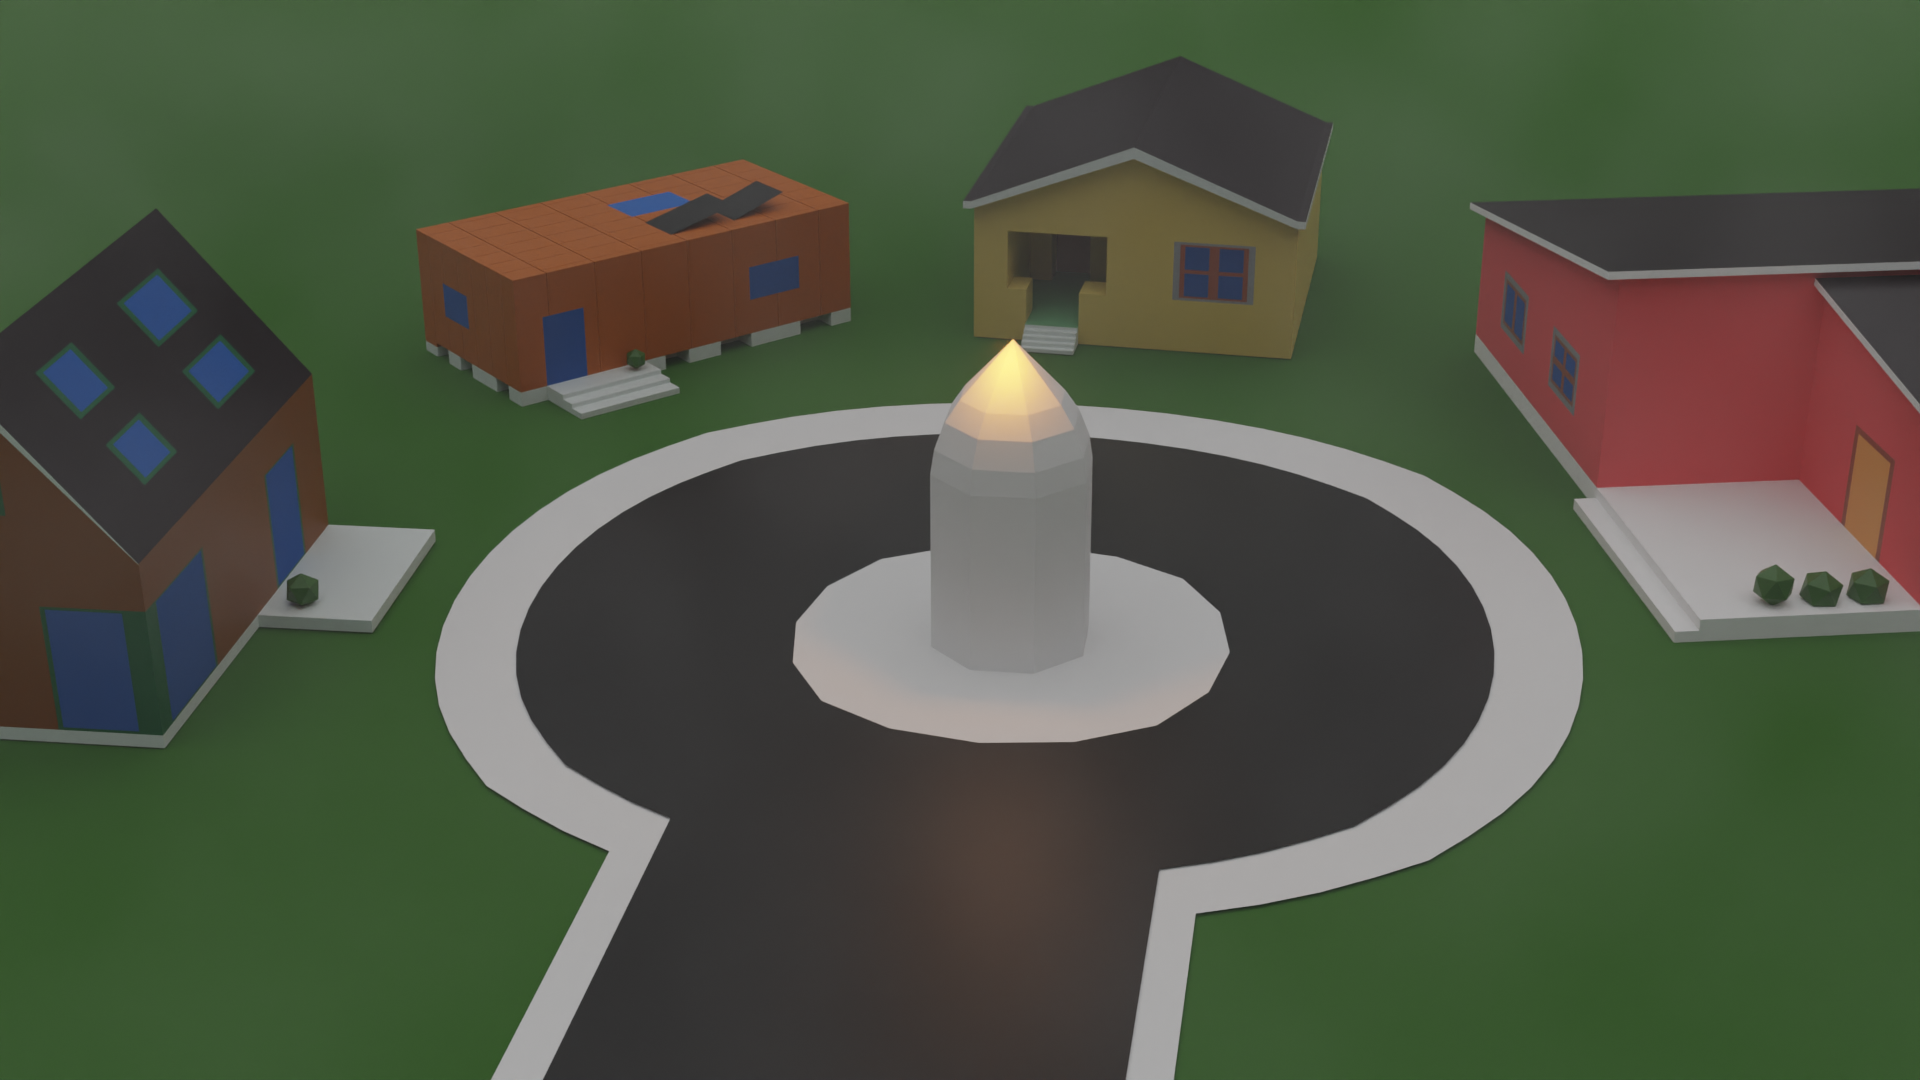
\includegraphics[width=.75\textwidth]{../img/district_3d_cycles_lights2.png}
  \caption{Centralized heat provider with glowing light.}\label{fig:culdesac}
\end{figure}

You go outside to see if there is anything you can do.
Apparently, engineers think alike, and all of your neighbors are gathered around the roundabout.
One of your neighbors has in her hands an open manual and reads it:
\begin{quote}
  «ERR706»: Consensus not reached.\\
  Restart the system and verify communication.
\end{quote}

The \dhn{} in question has a controller that solves an optimization problem to allocate the energy for each house.
However, some privacy questions were raised during its design, and the designers decided:
\begin{quote}
  «The controller must not know the exact needs of each resident.»
\end{quote}

After some discussion, they opted for a distributed method.
Each house was given one local controller to manage its temperature, and a coordinator controller was added to iteratively propose allocations for each building.

Just above the error code in the manual, you can take a glimpse of a diagram followed by a small text indicating the communication and the flux of information:
\begin{figure}[H]
  \centering
  \begin{tikzpicture}[font=\small,thick,node distance=3*0.6180cm and 0.6180cm,every node/.style=rectangle,
    mpcSmall/.style={fill=mpc_agent, minimum height=0.6180*2cm, minimum width=2cm},
    coordinator/.style={fill=mpc_coordinator, minimum height=0.6180*3cm, minimum width=6cm},
    ]

    \node[draw, mpcSmall,] (block1) {\small House 1};
    \node[fill=none, draw=none, right=of block1,] (mult) {\bf $\dots$};
    \node[draw, mpcSmall, fill=mpc_agent, right=of mult,] (blockM) {\small House M};
    \node[draw, coordinator, below=of mult,] (coordinator) {Coordinator};

    \draw[-latex,line width=1pt] (block1.south)+(0.4,.0) -- ( coordinator.north -| {$(block1.south)+(0.4,.0)$}) node [right,midway] {$\lambda_{1}$};
    \draw[latex-,line width=1pt] (block1.south)+(-0.4,0) -- (  coordinator.north -| {$(block1.south)+(-0.4,0)$}) node [left,midway] {$\theta_{1}$};
    \draw[-latex,line width=1pt] (blockM.south)+(0.4,.0) -- ( coordinator.north -| {$(blockM.south)+(0.4,.0)$}) node [right,midway] {$\lambda_{M}$};
    \draw[latex-,line width=1pt] (blockM.south)+(-0.4,0) -- (  coordinator.north -| {$(blockM.south)+(-0.4,0)$}) node [left,midway] {$\theta_{M}$};
  \end{tikzpicture}
  \caption{Exchange between local controllers and coordinator.}\label{fig:ex_exchange_agents}
\end{figure}

\begin{quote}
  \raggedright
  Allocations $\theta_{i}$ are proposed for each house by the coordinator.
  The local controllers respond with indices $\lambda_{i}$ to indicate satisfaction. Allocations are updated based on these indices until a consensus is reached.
\end{quote}
Today was not the case.

You and your friends verify the communication cables.
Everything is intact. You restart the system.
Lights turn off. Some seconds pass, and the orange LED turns on again.
The same error.

You try to debug the problem.
Fortunately, the program has an open data policy for the period of tests.
You look into the historical data but have too much data to grasp something valuable.
A friend gives an idea:
\begin{quote}
  -- What if we compare the same day of the week of the last 10 weeks? We can accumulate a loss function that depends on the deviation from the setpoints.
\end{quote}

«What a nice idea! Why didn't I think of this before?», You think.
\begin{quote}
-- I don't know if it is really a good idea. Maybe it is some internal error in the coordinator program.
\end{quote}
says your neighbor of house $1$.

You open a terminal in the central computer, anyway.
You can hardly feel the tips of your fingers touching the keyboard.
You filter the logs. Calculate the deviations and compute the loss functions for each house. You use the parameters of each house given by the manual, kindly lent by your colleague.
You also sum the functions for all houses giving a global loss function.
You plot the points and smooth the curves.
\begin{figure}[H]
  \centering
  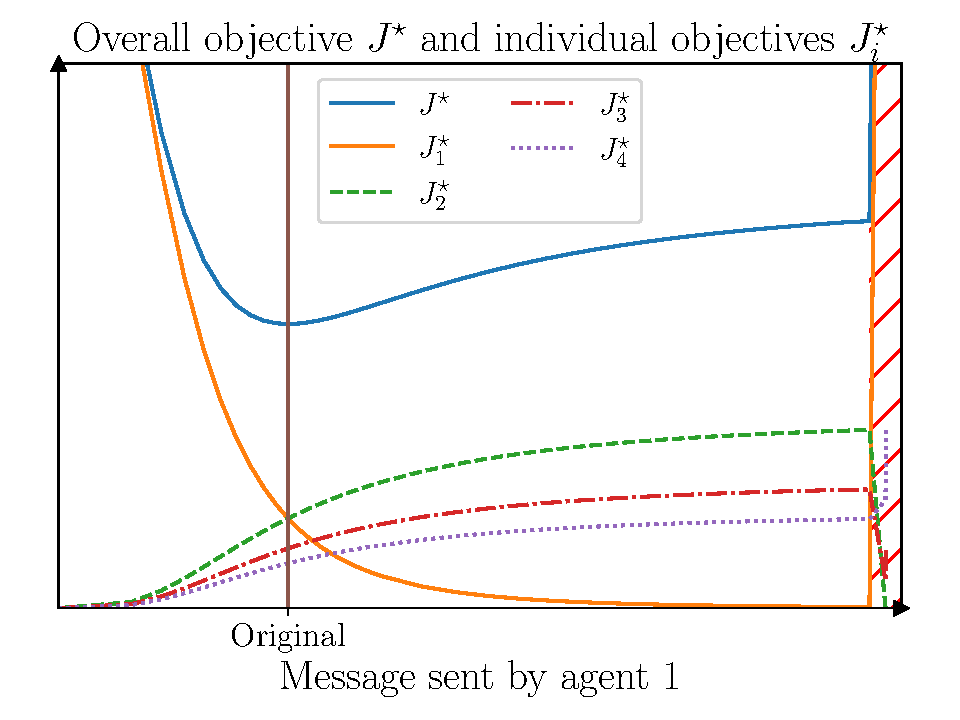
\includegraphics[width=.5\textwidth]{../img/qualitative_example.pdf}
  % ./docstheseplot -o ../../docs/img/quantiteAvecTriche4 -i  ../../data/matlab/tricheQuantite/dmpcQuantity4systemsTriche_.mat --quantiteAvecTriche4
  \caption{Plot of local and global loss functions from last 6 weeks.}\label{fig:change_in_j}
\end{figure}

\begin{quote}
  A-ha! Against facts, there are no arguments!
\end{quote}
You see the global function increasing after a given day. The increase rate steadily decreased until yesterday, when everything went awry.
You highlight it by hatching the area in red.
Your house, the house number $4$, has increased its function. And all other houses too. Wait! House $1$'s function decreases.
You show the plots to your neighbors, who afterward confront the resident of house number $1$.
After the indubitable proof, he finally breaks down and tells the truth.
\begin{quote}
  \raggedright
  Okay, okay. It was me. Some time ago, after studying the exchanges between my house and the coordinator, I realized something.
When my house sent increasing values of $\lambda_{i}$, the following allocations $\theta_{i}$ were greater.
  So I changed my circuit by adding an amplifier to increase my resources.
  You guys know I'm not used to these cold temperatures.
  I began with a small amplification.
And as no one noticed and the days were getting colder, I increased the amplification every day a bit.
  Everything went smoothly until today.
  And I would have gotten away with it, too, if it weren't for you meddling fellow engineers!
\end{quote}
The greediness of the neighbor shifted the negotiation so he could receive more resources.
Still, he was so greedy that the system could not find a consensus at some point.

You and your friends remove the said amplifier, file a complaint to the program organizers against the unethical colleague, and file a bug, showing the system's vulnerability.

After this day, you decide to make the system more resilient to such attacks, preventing their effects.
But first, you must catch up on the lost sleep hours and study the security of \cps{}.

\section{Motivation and Contributions}
Although the example given is ludic, it presents possible effects of attacks and malfunction in a \cps{}: Loss of optimality and eventually breakdown of the control strategy.

While one of them can sometimes be acceptable (depending on the suboptimality), the other is absolutely inadmissible, principally when we are talking about \cps{} that are essential for the population.
The consequences of non nominal behaviors may impact important parts of the life of the population and can even endangered it.

A bibliometric study~\cite{ZacchiaEtAl2019} shows how awareness on security of \cps{} has been raised.
This awereness was sadly motivated by many examples of attacks and faults all around the world in the last two decades.
Some examples are the Brazilian blackouts in 2010~\cite{Conti2010}, the Stuxnet attack on an Iranian uranium enrichment plant in 2011~\cite{Langner2011}, attacks in Ukrainian Power System in 2016~\cite{Bindra2017} and other~\cite{DingEtAl2018,DibajiEtAl2019}.

The main motivation of this work is to study attacks in \cps{}.
Focusing on \cps{} controlled by a \dmpc{} framework.
And using the knowledge gathered throughout the study to reduce the effects of the attacks as much as possible.
And to guide us on the quest to minimize them, we can raise some questions:

\simplebox{
  \begin{itemize} \bfseries
    \item Can we detect the attack?
    \item Can we identify the ill-intentioned agent(s)?
    \item Can we mitigate the effects of the attack?
  \end{itemize}
}
This work has as objective to answer these questions, at least for specific cases which will be formally presented.

To understand and answer those questions, we divide this work into two parts.

\paragraph{Part~\ref{part:mpc_intro}} It serves as a gentle introduction to \dmpc{} design, security and attacks.

For an unfamiliar reader, Chapter~\ref{sec:decomposing_mpc} explains what is a \mpc{} to begin with and shows some of the challenges to decompose it.
Chapter~\ref{sec:topology_trust} discuss possible topologies used for those decompositions.
In Chapter~\ref{sec:anomalous} we define anomalous behaviors, give some examples, categorize them and present some methods used to prevent and combat them.

\paragraph{Part~\ref{part:safe_dmpc}} It contains the contributions of this work.

Chapter~\ref{sec:primal_decomposition} presents the decomposition studied in this work (primal decomposition). We present its vulnerabilities and how they can affect the performance of the system. Here we formalize the Example given in the story giving it a more quantitative approach.
Once we know the vulnerabilities and possible effects of attacks, we divide the mitigation problem into more manageable parts.
\\ First in Chapter~\ref{sec:safe_pddmpc_eq}, we analyze an unsophisticated problem, so we can assess the difficulties that can be found when solving the mitigation problem. From the analysis of the problem we propose a detection and mitigation mechanism, followed by an academical example to illustrate its functioning.
\\Then, in Chapter~\ref{sec:safe_pddmpc_ineq}, we analyze a similar problem but with a twist. As we will see, just one small modification on the initial problem can increase exponentially its complexity.
From the analysis of the newly-found problem we propose a similar strategy, but with adequate modifications to contain the exponential nature of the problem.
\todo{\\Finally, we continue in Chapter~\ref{sec:safe_pddmpc_ineq_reconst} the methodology and explore some more properties to create a less conservative strategy.}
\\Then, we conclude this work in Chapter~\ref{sec:conclusion} with a discussion about the results found during this study, benefits as well as shortcomings. Some of this discussion leads to open questions which can incite new works.

\subsubsection{Contributions}
We can list as a minor contribution of this work the study of vulnerabilities of Primal decomposition-based \dmpc{}, which wasn't studied to the best of our knowledge,
And as main contributions \todo{three} mitigation strategies different kind of systems with increasing complexities.

The most simple strategy, for systems where the local demands (resources needed) are greater than total resources available, here called \textbf{Scarce Systems}.

\todo{And }A exponentially more complex system, where local demands respect only some constraints which we can use to get scarcity information by means we call \textbf{artificial scarcity}.

\todo{And finally a more general and complex, when there is no scarcity information available}
% Since those questions are still open, this work has as objective to discuss these questions by analyzing the recent literature and schematizing the security in decomposition methods for Model Predictive Control passing by the following items:
% \begin{itemize}[label=$\bullet$]
%   \item decomposition methods;
%   \item topology;
%   \item points of vulnerability;
%   \item how malicious agents can benefit from such vulnerabilities;
%   \item effects on the overall system;
%   \item possible ways to mitigate.
% \end{itemize}
% We use some conclusions of the discussion to develop safe algorithms for a \dmpc\ framework.

\section{Publications}
The work and discussion presented in this thesis yielded the following publications
\begin{itemize}
  \item Published
        \begin{description}
          \item[\cite{NogueiraEtAl2021}] Conference article for the SysTol'21
          \item[\cite{NogueiraEtAl2022}] \todo[correct citation]{} Conference article for the NecSys'22
        \end{description}
  \item Under Review
  \item In Preparation
\end{itemize}



% \chapterEndOrnament

\end{document}
